\section{Final Design}\label{sec:finalDesign}

The final goal is the have an end-effector velocity of 9.47 $\frac{m}{s}$ at $45^o$.  
The key-frame method was tested to throw at 4.8 $\frac{m}{s}$.  
To increase the end-effector velocity the upper body motion was kept unchanged but the lower body added a stepping motion with its legs.
The stepping motion consists of lifting the left foot up, pushing forward with the right and move the left forward 10 cm.  
Stepping with your non-dominant foot, and pushing with the dominant, when throwing overhand is common practice to increase the distance you can throw a ball.  
Jaemi Hubo throws with its right hand and steps with its left.  
This increased the end-effector velocity from 4.8 $\frac{m}{s}$ to 7.1 $\frac{m}{s}$.
Fig.~\ref{fig:hubo-step} shows the stepping motion of the robot.

\begin{figure}[t]
  \centering
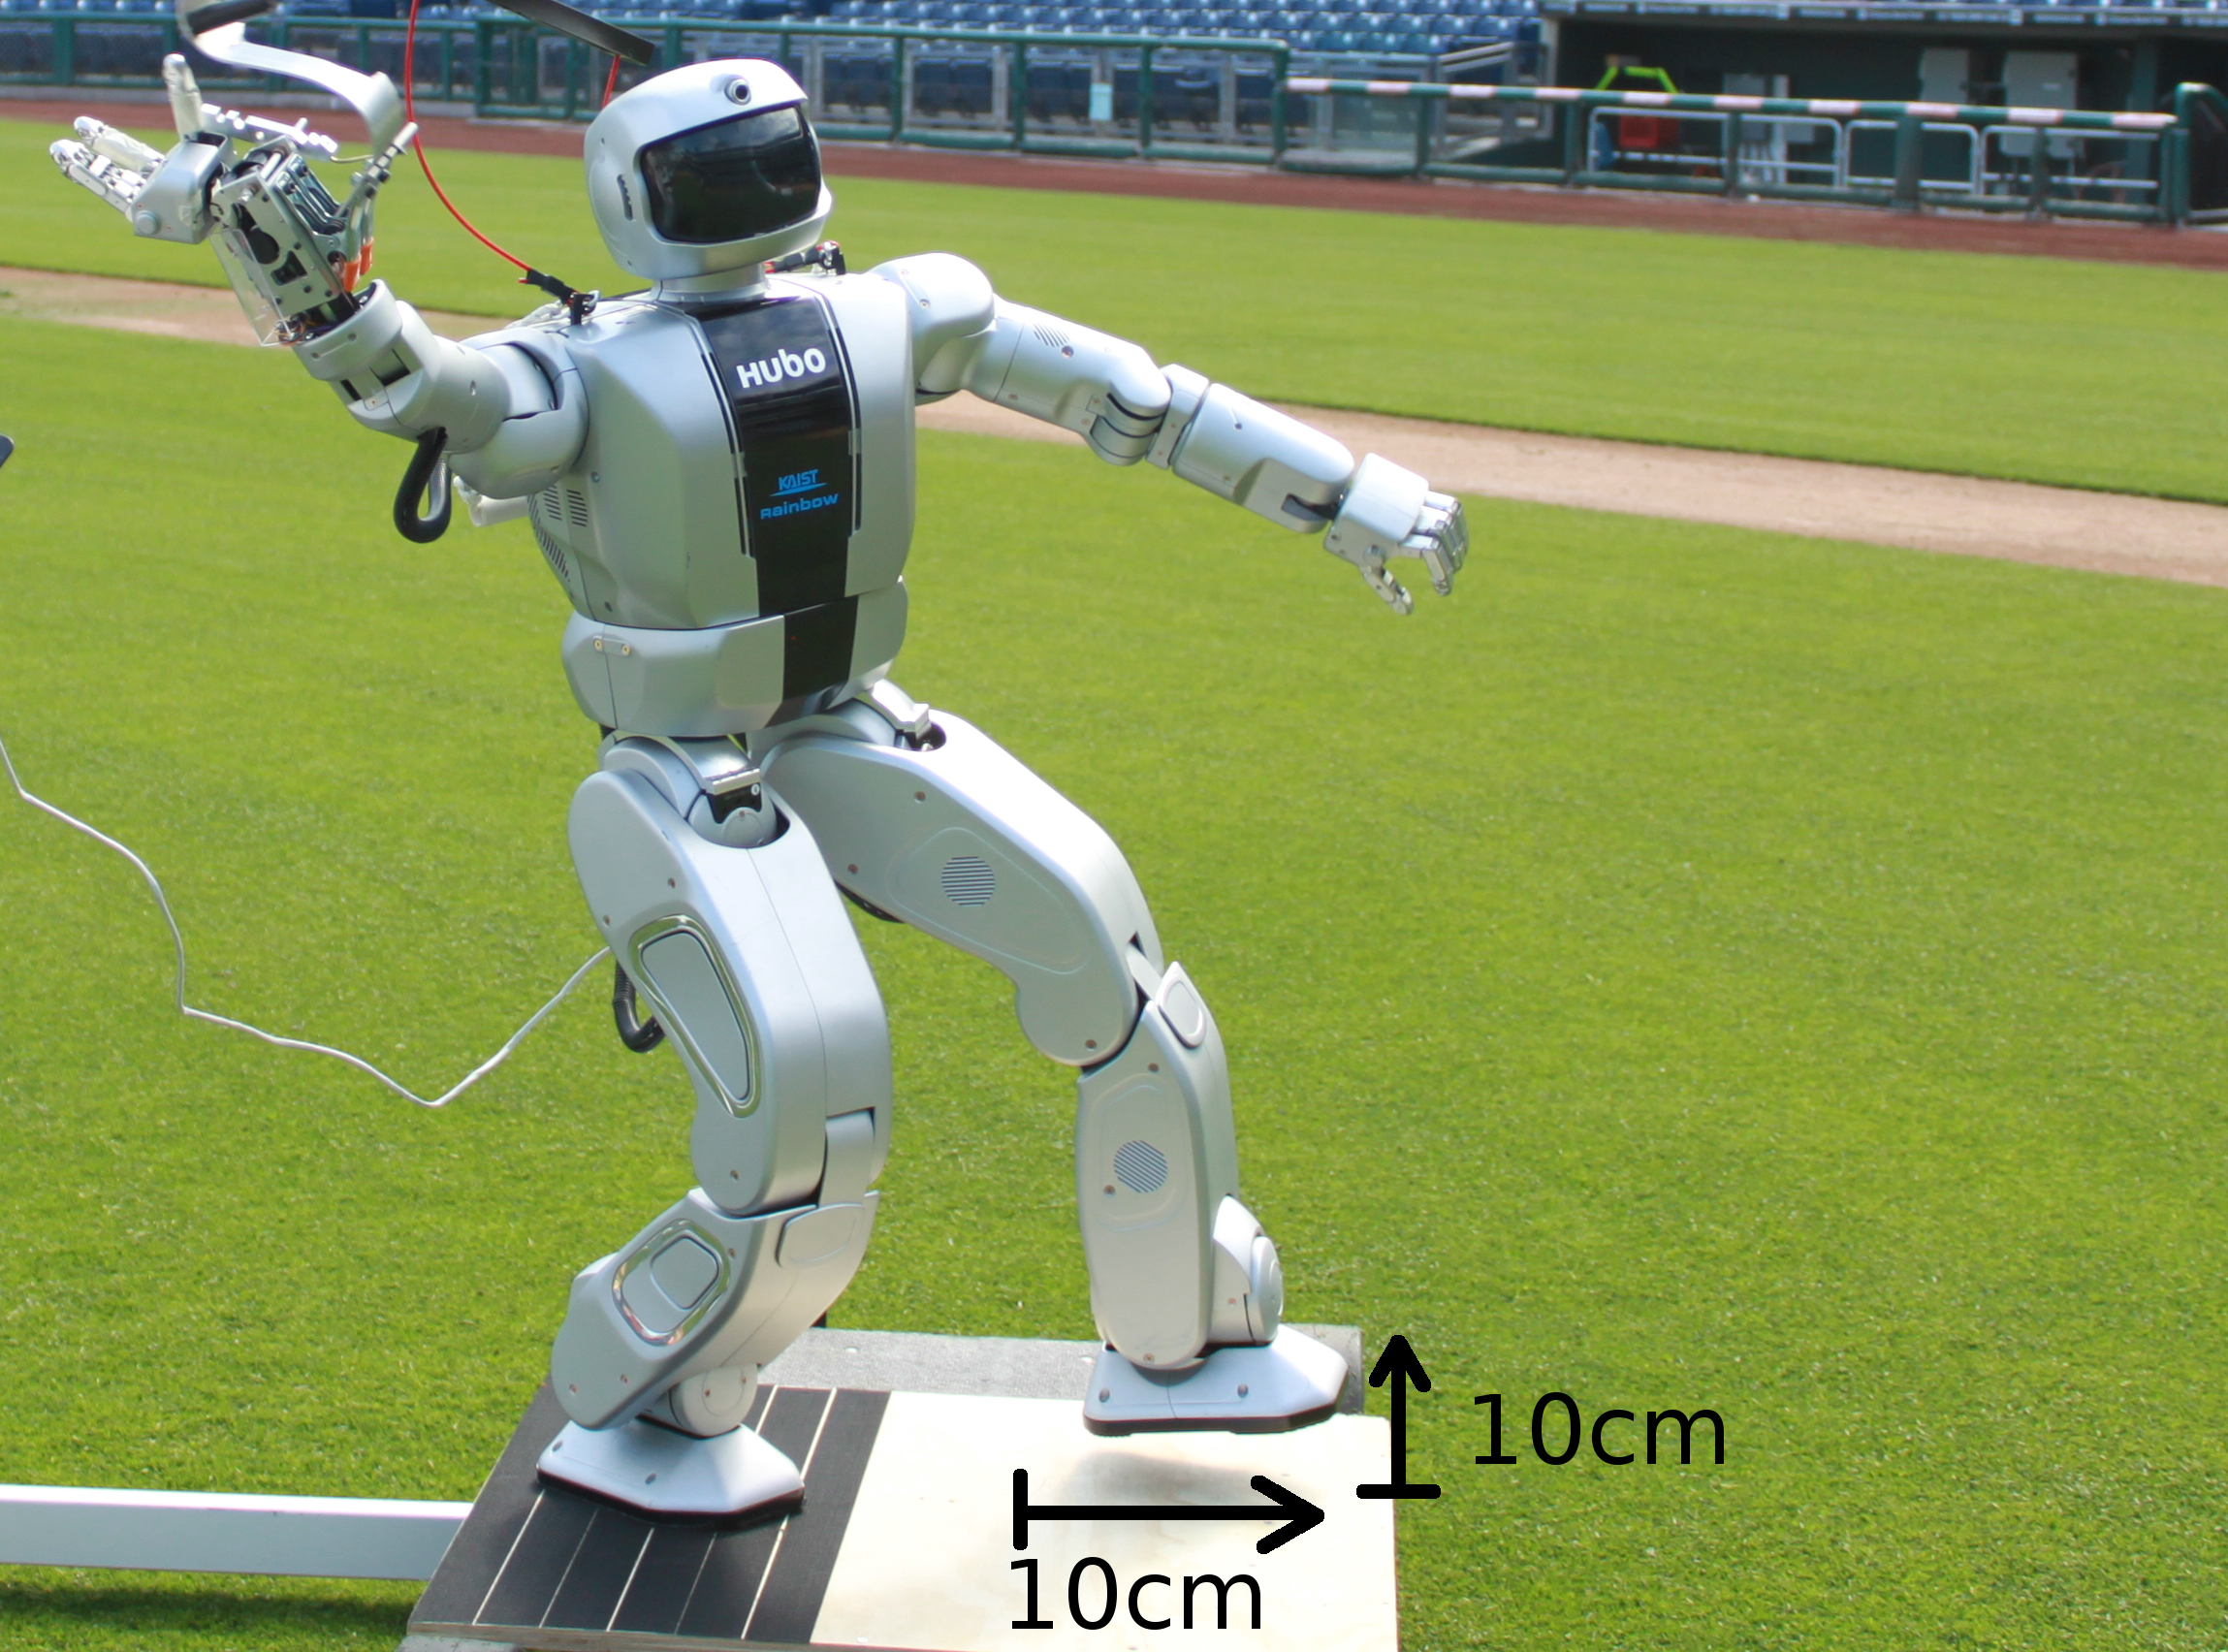
\includegraphics[width=1.0\columnwidth]{./pix/throwPractice.png}
  \caption{Hubo stepping 10 cm up and forwards increasing the end effector velocity by 2.3 $\frac{m}{s}$.}
  \label{fig:hubo-step}
\end{figure}

The addition of pushing off with the right foot and stepping forward introduced two problems.  1) The ZMP criteria is not satisfied throughout the motion and 2) the right foot would slip when pushing its body forward.  
To avoid slip \textit{hook and loop} was paced on the bottom of the right foot (non-dominant) and on the throwing platform.  
This did not permanently attach the robot to the platform but it did allow for more friction between the foot and the ground.
This allowed the balancing controller to function adequately for the short step and maintain stability.
The platform was added to ensure a more consistent ground for the robot to balance on than the baseball field can inherently provide.

\begin{figure}[t]
  \centering
\includegraphics[width=1.0\columnwidth]{./pix/finalSpring1.png}
\includegraphics[width=1.0\columnwidth]{./pix/finalSpring2.png}
\includegraphics[width=1.0\columnwidth]{./pix/finalSpring3.png}
  \caption{Spring loaded mechanism test launching the baseball.  Top: Pre-launch.  Middle: Launch.  Bottom: Pos-launch.  The mechanism added 3.0 $\frac{m}{s}$ to the end-effector velocity at its release point.}
  \label{fig:hubo-spring}
\end{figure}

\begin{figure*}[t]
  \centering
\includegraphics[width=1.0\textwidth]{./pix/preThrow2.png}
  \caption{Frame overlay of the Hubo throwing overhand a distance of 10 m (32.8 feet) with a release angle of 40$^o$ and a tip speed of 10 $\frac{m}{s}$.  Captured at 20 fps with a shutter speed of 1/30 sec.  Each of the white dashes of in the image is the actual baseball as picked up by the video camera.}
  \label{fig:hubo-throw-test}
\end{figure*}

An additional 2.5 $\frac{m}{s}$ was needed to give a proper throw.  
Borrowing from the GRASP Lab and their high powered pneumatic wrist on their PhillieBot, a spring loaded mechanism was added to Hubo's wrist, see Fig.~\ref{fig:hubo-spring}.
The addition of this mechanism allowed the robot to achieve an end-effector velocity magnitude of 10 $\frac{m}{s}$.
Fig.~\ref{fig:hubo-throw-test} shows a frame overlay of the the Hubo throwing a regulation baseball 10 m (32.8 feet).
Fig.~\ref{fig:hubo-throw} shows the same throw at Citizens Bank Park on April $28^{th}$, 2012.




